
\section{Experiments and Simulations}

\section{The minimal viable product}
The minimal viable product (MVP) is a version of a new product that includes only the essential features necessary to meet the needs for initial testing. The goal of an MVP is to validate the product idea with minimal resources and gather feedback for future development. In figure \ref{fig:MVP} you can see the result of the MVP and in figure \ref{fig:MVPpipeline} you can see the pipeline that is used for the MVP.

\begin{figure}[!htp]
    \centering
    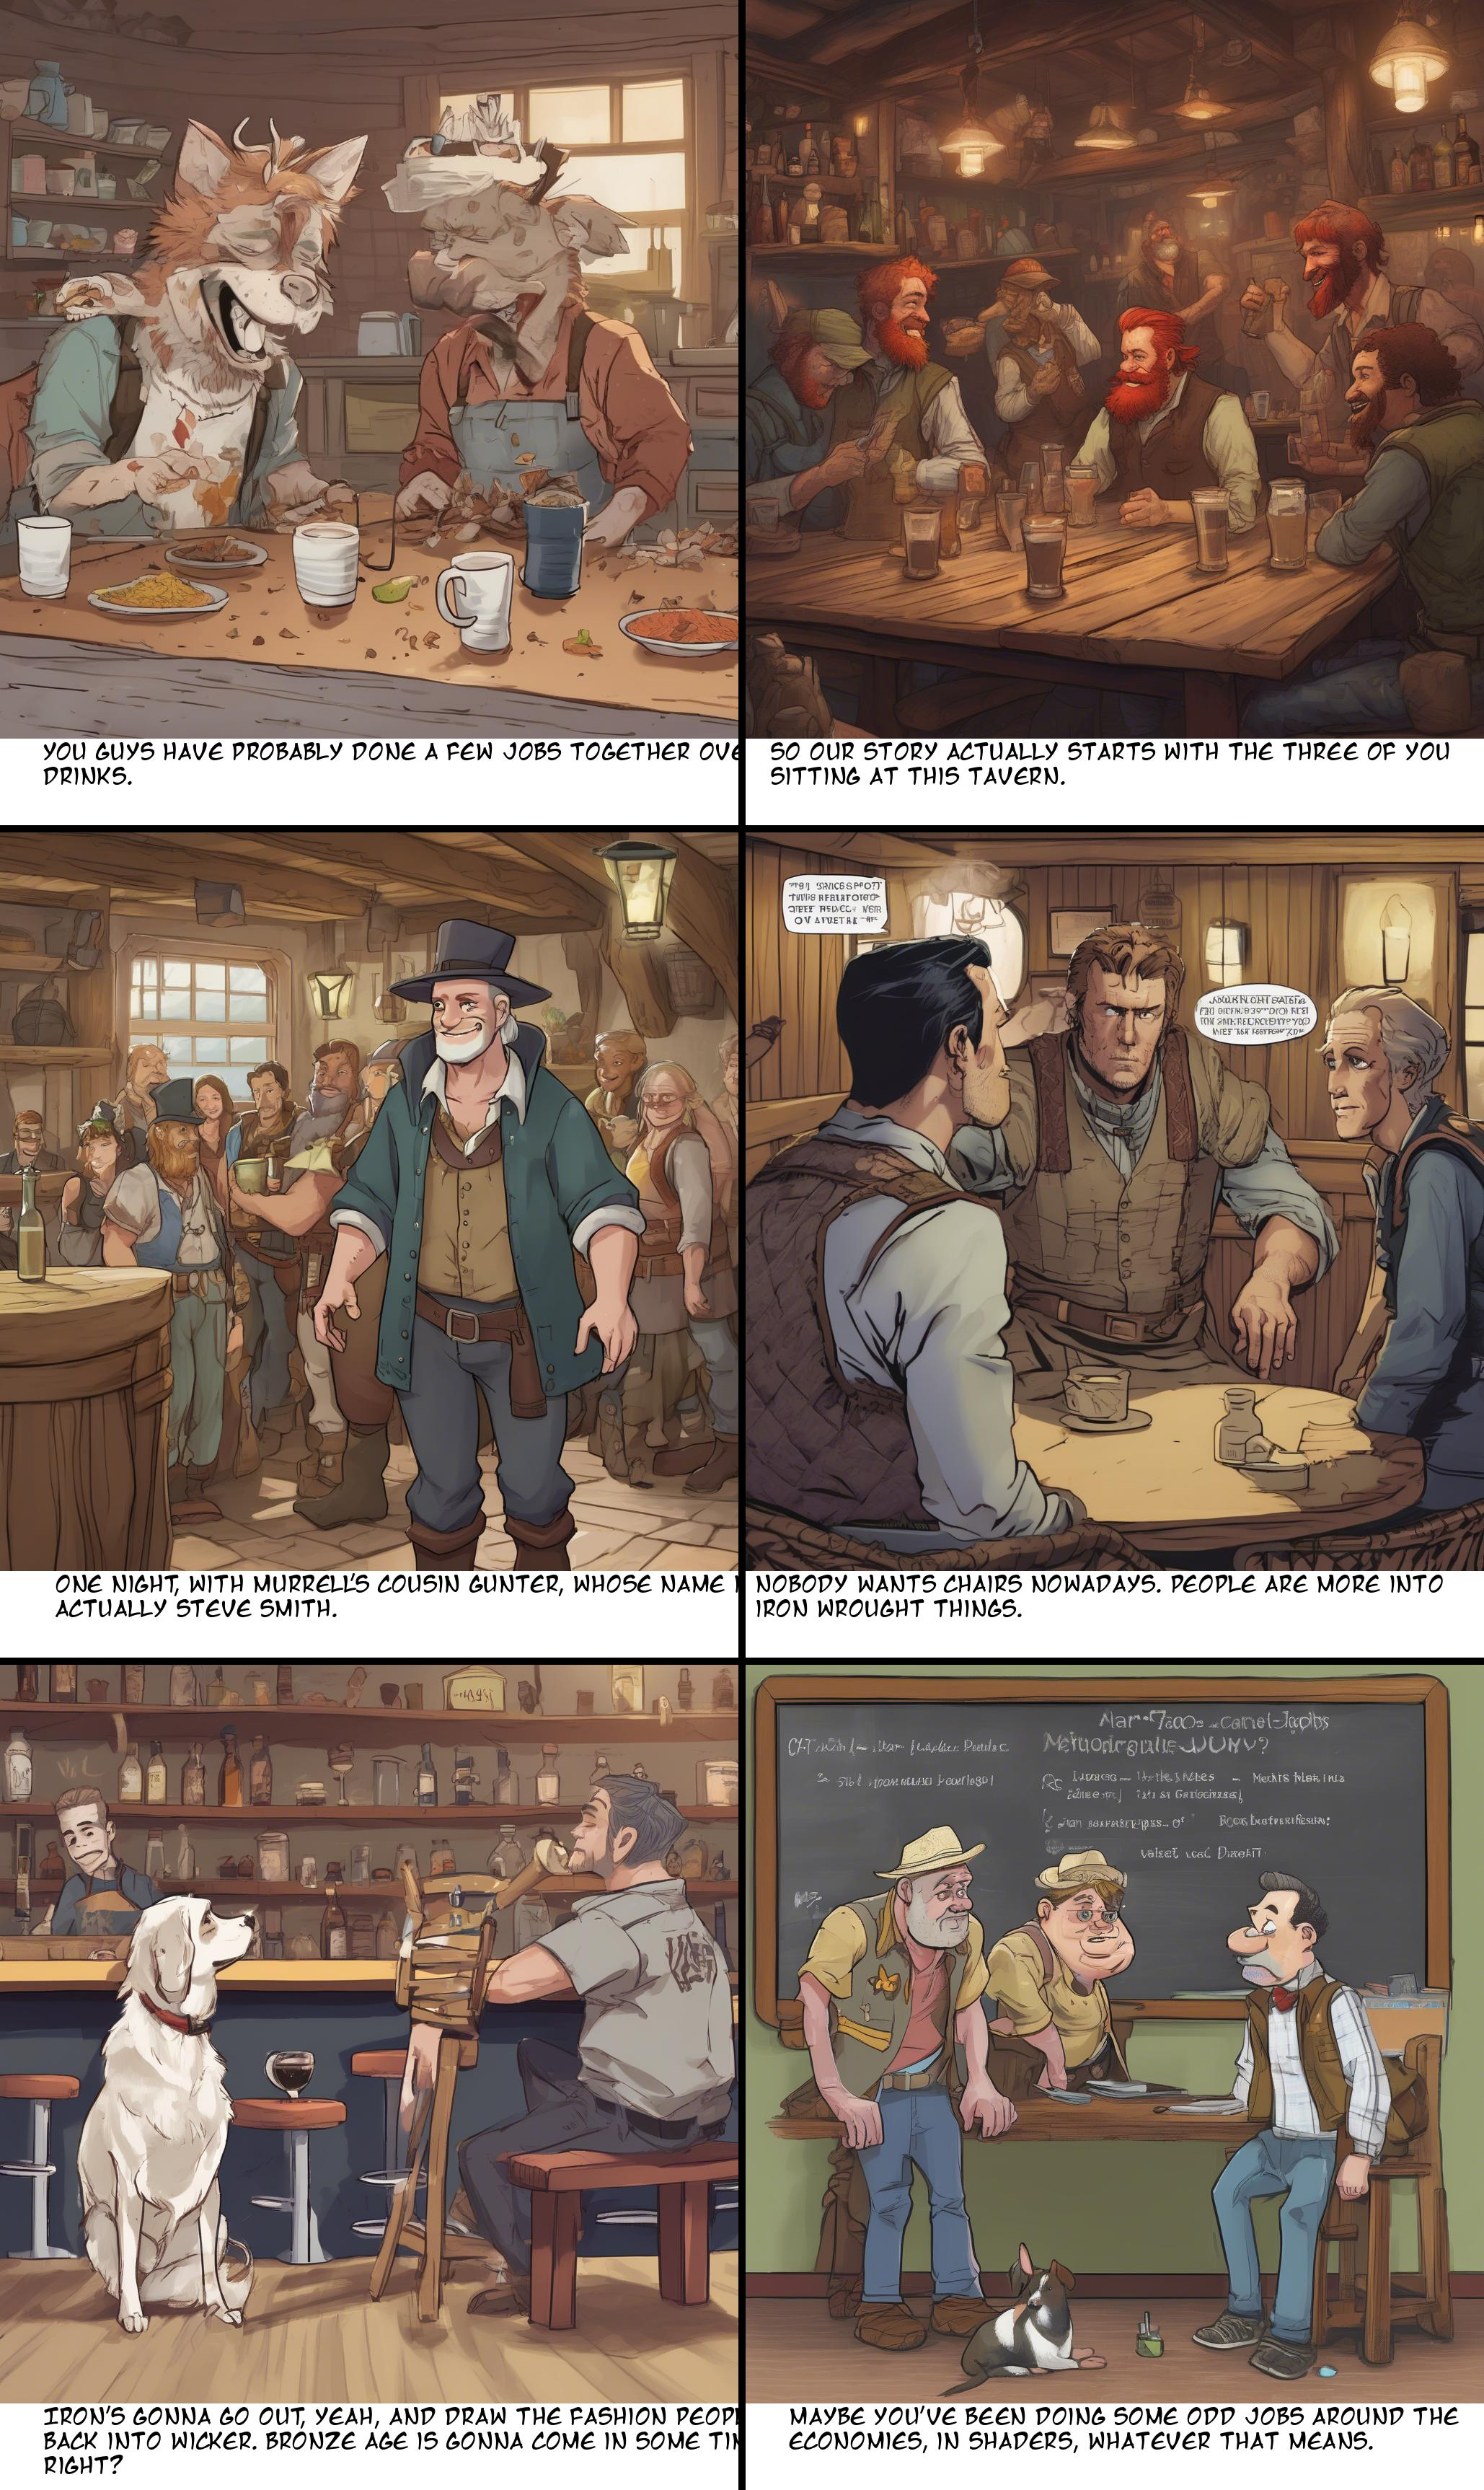
\includegraphics[scale=0.2]{images/mvpTTRPGtoComic.png}
    \caption[The minimal viable product]{The minimal viable product}
    \label{fig:MVP}
\end{figure}

\subsubsection{MVP pipeline}
The MVP pipeline has 4 steps of processing to go from audio recording to comic book. First Whisper Turbo transcribes the audio recording to raw text. Then Llama 3.1 converts the text to a comic book script. The script is then processed by Stable Diffusion XL to generate the comic book panels. Finally, the panels are assembled into a comic book format using a custom python script. The pipeline is shown in figure \ref{fig:MVPpipeline}. The audio recording is a single track recording of a tabletop role-playing game session. The prompt used for Llama can be seen in listing \ref{lst:MPVLlamaprompt}. This prompt generates a description of the panel art and a line of dialogue or narration for each panel. The output is a JSON array of objects, where each object contains the panel art description and the text. The panel art description is then given to Stable Diffusion XL to generate the image with no other instructions. The text is used as a caption for the image. The images are then assembled into a comic book format using a custom python script which generates a PDF file with the images and captions.

\begin{lstlisting}[style=jsonstyle, caption={Prompt for Comic Book Script Generation}, label={lst:MPVLlamaprompt}]
You are given a segment of a Dungeons & Dragons session transcript:

Session Content:
{content}

Your task is to transform this into a comic book script, broken down into individual panels.

Each panel must include:
- A detailed visual description suitable for image generation (key: "panel art")
- A line of dialogue or narration (key: "text")

Instructions:
- Structure the output as a JSON array of objects.
- Each object must contain exactly two keys:
- "panel art": A vivid, standalone description of the panel art. Include setting, characters, action, and mood.
- "text": A single line of spoken dialogue or narration. Rephrase as a proper sentence if needed, but keep the meaning true to the original session.
- Process the entire input and split it into as many panels as necessary.
- Do **not** include any additional explanation, commentary, or text outside of the JSON array.

Output only a valid JSON array. Example format:

[
{
    "panel art": "A dimly lit tavern filled with laughing patrons. Magnus, a red-bearded human, clinks mugs with Taco and Merle at a wooden table.",
    "text": "So our story begins with the three of you sitting at this tavern."
},
{
    "panel art": "Close-up of Magnus, his face lit by candlelight, a sheepish grin on his face.",
    "text": "Nobody wants chairs anymore. Everyones into wrought iron now."
}
]
\end{lstlisting}

\subsection{Lessons learned}
The MVP was a success in terms of validating the product idea and gathering valuable knowledge about the product requirements and limitations. In this section lessons learned are described in detail and it is discussed how these lesson will be implemented in the next iteration of the product.

\subsubsection{Art}
The first thing one might see when looking at the MVP output is the art. The art quality is low, it is not very detailed, the characters are not very expressive and the art style is very inconsistent. There are also a lot of generative AI artifacts, like weird faces and inconsistent human anatomy. Furthermore all these panels are situated in the same tavern, but the there is no consistent setting. All these panels also describe 4 different characters and but there is no consistent character design between panels.

\subsubsection{Text}
The text has one obvious flaw of clipping outside of the image which is something that needs to be fixed. Other then that when reading the text it is noticeable that it is not really character dialogue, but things the players are saying. Some of the text is player to player dialogue and not in character dialogue which is something that needs to be filtered out. The text also does not make any since in term of story structure. These are just lines of text.

Looking the entire transcription of the tabletop role-playing game session it can quickly be seen that there is no structure to the text, making it extremely difficult for an LLM to make anything meaningful out of it. Figure X is a expert of the transcript where you can see that it is just a consistent stream of text without any structure.

\subsubsection{Composition}
All the panels have a similar camera angle and composition.

\subsection{Solutions}
In this section possible solutions are discussed which will be implemented for the next iteration of the product. The goal is to improve the quality of the art, text and composition of the comic book panels.

\subsubsection{Art}
Stable Diffusion is a pre-trained model that is made to work for any art style, to create a consistent art style you could write a art style prompt, however this creates issues with the token limit that stable diffusion has. The proper way to do this is by using a loRA (Low-Rank Adaptation). LoRAs are a way to fine-tune a pre-trained model on a specific task or domain. In this case, a LoRA can be trained on a specific art style to create a consistent art style for the comic book panels. This will also allow for more detailed and expressive characters. The LoRA can be trained on a dataset of comic book panels in the desired art style. The LoRA can then be used in Stable Diffusion to generate the comic book panels with the desired art style. However since training a LoRA is outside of the scope of this project a pre-trained LoRA from civitai.com will be used. This also comes with the benefit that any LoRA can be used to generate any art style wanted by the user.

\subsubsection{Character consistency}
To create consistent characters between panels there are 5 different approaches that can be taken. LoRA's can be used for each character creating a very consistent character design. This does require each character to have a LoRA trained on it meaning that you need to have art of the character to start with. This would also mean that the images would be generated with multiple AI's generating images and then having to combine them. 
The second option would be image-to-image reference chaining. With this method you give SDXL a reference image of the character and then generate the panel with the character art as a reference. 

The easiest and least consistent manner would be to use consistent prompting. This means that you give the same prompt for each panel with the character description in it. This will however not create a very consistent character as each iteration of the prompt will interpret the prompt differently. Resulting in many different smaller inconsistencies. This however would be a good step if the other methods would be too time consuming to implement. It would most likely require two iterations of generating the image, one for the character and one for the panel art. As the number of tokens in the prompt would be too high to generate the panel art and character art in one go.

Inpainting is a technique where you alter part of an image so that it fits your desired effect. You select an area of the image and then fill it in with a new image, generated by AI. This gives you a way to control very specific parts of an image and finetune an image. Normally this requires a lot of manual work where you have to cut out the area which has to be painted in. It would however be possible to use computer vision to detect the character in the image and then use that as a mask for the inpainting. This might result in a very good solution, but there are potential issues with multiple characters in the same panel.

Lastly an option could be using ControlNet. This is a technique where you use a pose reference images to control the pose of the character in the image.

In the end it would most likely be best to use most of the above techniques in combination to create the best possible result. Create a LoRA to have consistent character art, use inpainting to place the art on top of the panel art and use ControlNet to control the pose of the character. 
\subsubsection{Scene consistency}
In the current comic page of the MVP each scene is taking place in the same tavern, but the tavern is not consistent between panels. Most solutions given in the previous section on character consistency could be used here as well, however as there are way more variables possible for locations creating a LoRA is impossible and would defeat the purpose of using AI. You could however let AI create images of a tavern and the use those images as reference materials for future uses of that tavern. Meaning you need to keep track of scenes and locations so that you can bring back the same panels in later parts of the comic book. 

\subsubsection{Text}
To fix the text that is in the panels of the comic books the first step would be to fix the transcript of the game session. As is always the case with AI: Garbage in is garbage out. Fixing the transcript will also have effect on the other parts of the comic book, as there will be a clearer structure to the text which can be used in a better way to generate images and create structure between panels. To fix the transcription there are a few that need to be taken.

After transcribing the audio recording with whisper there are 3 steps we can take to increase the usability of the text. First we need to use a Punctuation and Capitalization Restoration model to fix the text by adding punctuation and capitalization to the text. This will make the text more readable and easier to understand. The second step would be to use Speaker Diarization to identify the different speakers in the text. This will benefit with knowing who said what at which time and allows to have accurate charact dialogue. Furthermore this makes it so that the Game Master can be identified as someone who plays multiple characters. A tool to do this is Pyannote Audio, an open-source toolkit written in Python for speaker diarization. Lastly combine the cleaned up whisper transcription with the speaker diarization to create a structured text file.

The next step is to then use an LLM to check all the text and identify what is character to character and what is player to player speech. Creating a clear divide between what does and what does not belong in the comic book. For the game master the same thing needs to happen, but then it is required to identify which character they are playing at that moment. Then an LLM would need to convert the text into real sentences which make sense in the context of the scene as something a someone in the English language would say.

\begin{figure}[!htp]
	\centering
	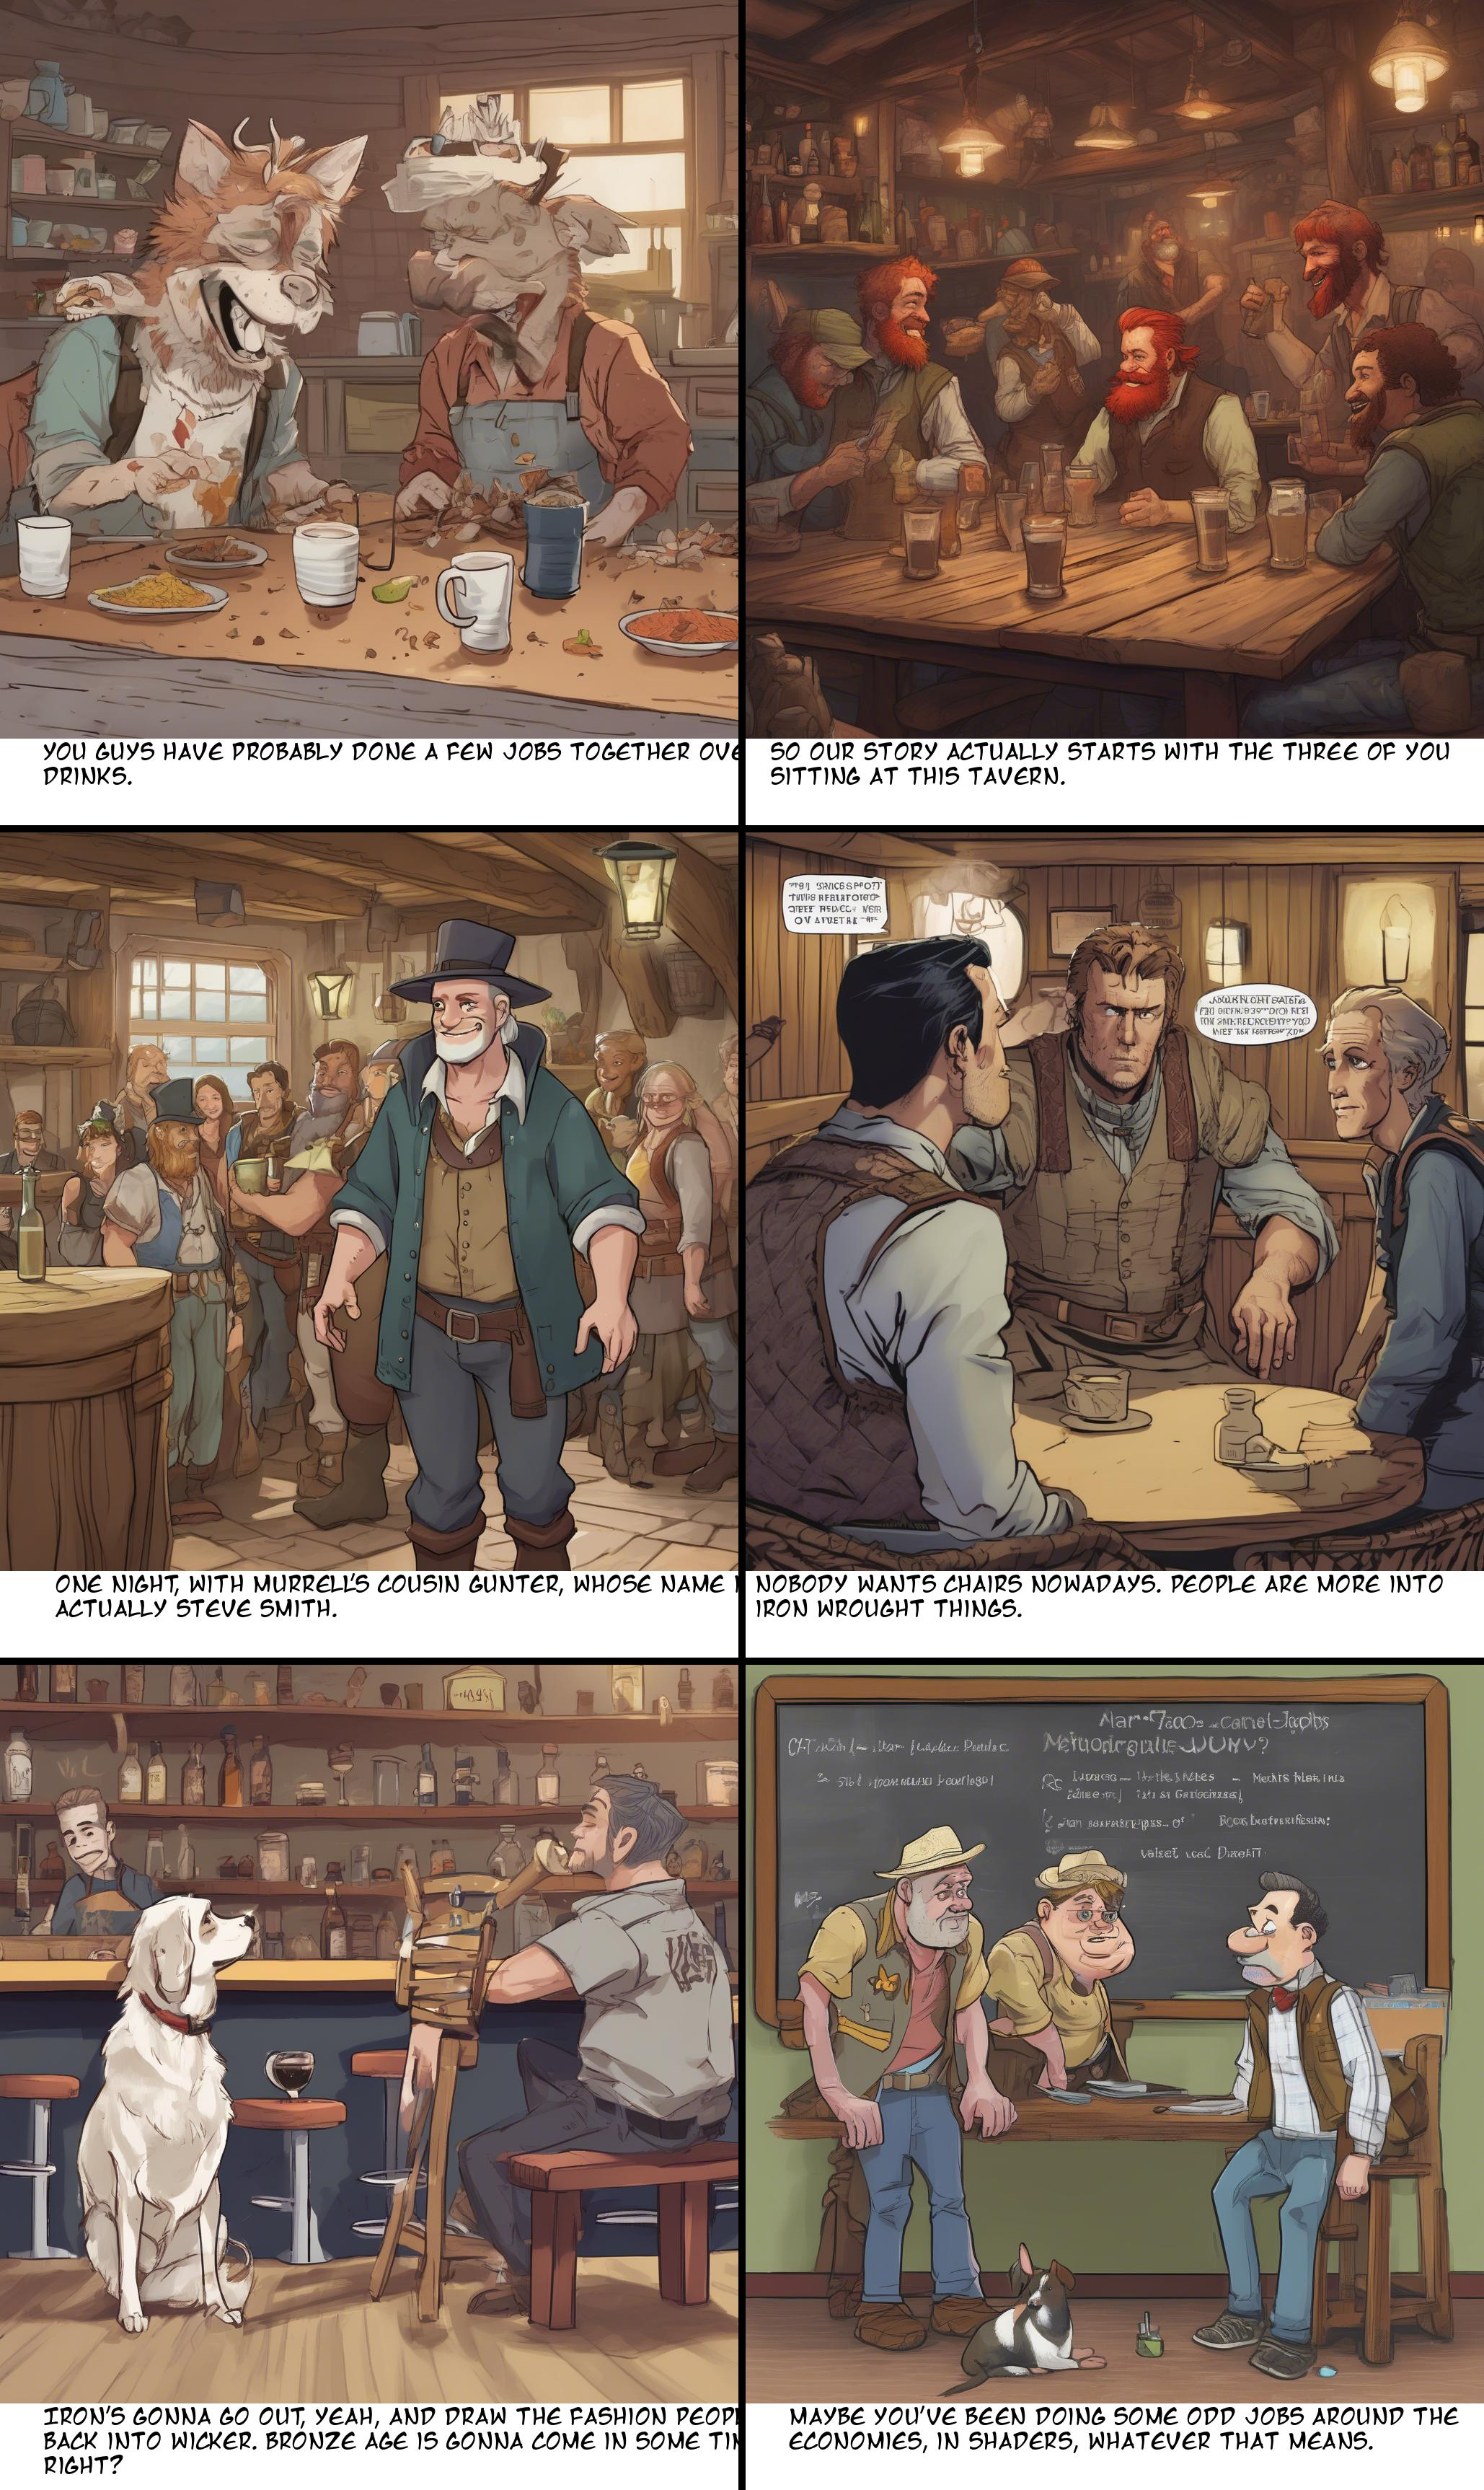
\includegraphics[scale=0.1]{images/mvpTTRPGtoComic.png}
	\caption[pipeline for the minimal viable product] {The minimal viable product pipeline}
	\label{fig:MVPpipeline}
\end{figure}

\subsection{The minimal viable product}

\section{Small experiments}

\subsection{The language of TTRPGs}
Models like Whisper are trained on a wide variety of audio data, however this is primarily normal language usage. Because of this I anticipate that there will be a large issue with transcribing many fantasy words and terms, thus a small experiment has been done to identify if this is truly a problem. For this experiment 10 fantasy creature names have been recorded and whisper transcribed these 10 names. Only 1 out of the 10 names were transcribed correctly and 2 out of 10 where almost correct \ref{tab:monster_names}. This is inaccuracy is a big issue when transcribing any fantasy game session as it will interfere with many important key moments and key names during a session/campaign. When the group meets a monster called a "Slaad" and Whisper transcribes this as "Nod" it will quite confusing to understand what is going on in the story.

To generate a accurate transcription of the names a custom model needs to be trained on specific fantasy words and terms, however this is way outside of the scope of this thesis. In addition it is also very difficult as Fantasy names are fantasy names for a reason and people can just come up with new names all the time. Integrating thousands of names however could still be valuable as it will most likely catch most cases.
\begin{table}[h!]
\centering
\begin{tabular}{|l|l|}
\hline
\textbf{Correct Name} & \textbf{Transcribed name} \\
\hline
Owlbear    & Halber     \\
Goblin     & Goblin     \\
Rakshasa   & Raksasa    \\
Dracolich  & Draco Lich \\
Quasit     & Kwasi      \\
Slaad      & Nod        \\
Drow       & Drought    \\
Illithid   & Illidan    \\
Cambion    & Kempion    \\
Ankheg     & Hank Man   \\
\hline
\end{tabular}
\caption{Comparison of monster names and whisper transcribed versions}
\label{tab:monster_names}
\end{table}

\section{Generating the comic book script}
The iterative design process of generating the comic book script after the MVP version was a crucial step to improve the quality of the comic book panels. From having a one-shot approach where we gave the entire transcript to the LLama 3.1 model, we moved to an adaptive panel generator which has a structured approach to data and keeps track of the context. In this section all the iterative steps are described and what did and did not work in chronological order.

\subsubsection{MVP}
For the MVP of the artefact the entire transcript of the tabletop role-playing game session was given to Llama 3.1 and see what it would generate. The LLM was asked: "You are given a Dungeons and Dragons session transcript. Convert it into a comic book script." This resulted in two results: The LLM crashed as the token limit was exceeded or it gave things that had nothing to do to with the input and hallucinated everything. A quick fix to this was to cut the transcript into smaller chunks of text which resulted in an interesting result as it actually gave a comic book script. It was given 2 scenes of text which where hand cut out of the transcript. However as the LLM was not instructed to give a structured output it was useless as every time the program was run it would give a different output. The last step was to create a structured prompt for the LLM which is the prompt in \ref{lst:MPVLlamaprompt}. This resulted in a consistent JSON format output which could then be used to generate images.

\subsubsection{Cleaning up the transcript}
When you feed an audio recording to Whisper it transcribes the audio as one long sentence. There is no punctation or any idea of sentences structure. This way it is impossible to keep track of who said what and when. To fix this the transcript needs to be cleaned up. The first step is to use a Punctuation and Capitalization Restoration model \cite{guhr-EtAl:2021:fullstop} to add punctuation and capitalization to the text. This will make the text more readable and easier to understand for an LLM. The second step is to use Speaker Diarization to identify the different speakers in the text. The tool used to do this was pyannote 3.1 \cite{Bredin23,Plaquet23}, an open source python library which is super easy to use and broadly used by people (15 million download per month). Lastly combine the cleaned up whisper transcription with the speaker diarization to create a structured JSON file. This new transcript file \ref{lst:sessionTrarnscriptJSON} is what created the foundation for the entire comic book generator.

\begin{lstlisting}[style=jsonstyle, caption={Session transcript JSON}, label={lst:sessionTrarnscriptJSON}]
{
    "panel_index": 0,
    "speaker": "SPEAKER_02",
    "text": "Our story actually starts with the three of you...",
    "start": 0.0,
    "end": 2.96
},
...
\end{lstlisting}

\subsubsection{Scene detection}

\subsubsection{Line based chunking}
Every line or every X lines

\subsubsection{LLM based chunking}
Scene cutting

\subsubsection{LLM based filtering}
Ask the LLM to decide if a line of text is player or character speech. Into giving it a chunk instead.

\subsubsection{Context aware LLM based chunking}

\subsubsection{Adaptive panel generating}